\documentclass[tikz, border=15pt]{standalone}
\usepackage{tikz}
\usetikzlibrary{calc, arrows.meta, positioning, shapes.geometric}

\definecolor{clientbg}{HTML}{FFF5F5}
\definecolor{clientborder}{HTML}{E53E3E}
\definecolor{idpbg}{HTML}{FAF5FF}
\definecolor{idpborder}{HTML}{805AD5}
\definecolor{meshbg}{HTML}{F0FFF4}
\definecolor{meshborder}{HTML}{38A169}
\definecolor{idtoken}{HTML}{DD6B20}
\definecolor{accesstoken}{HTML}{3182CE}
\definecolor{servicetoken}{HTML}{319795}

\begin{document}
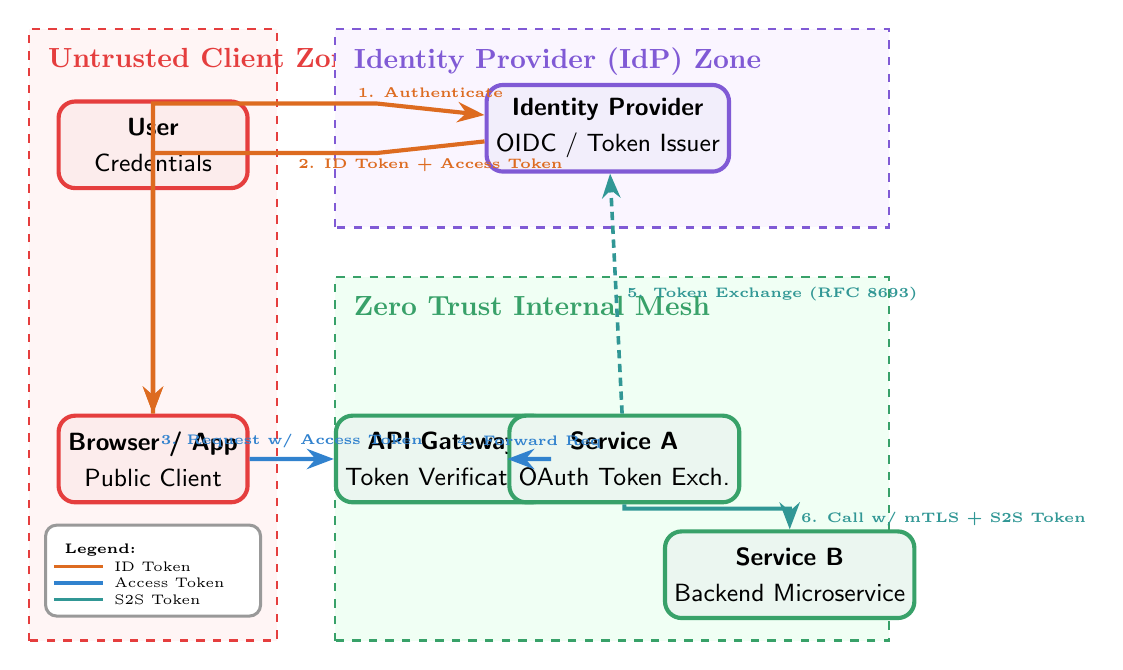
\begin{tikzpicture}[
    scale=1.05,
    >=Stealth,
    line width=1.1pt,
    font=\sffamily\small,
    block/.style={draw=#1, fill=#1!10, rounded corners=6pt, line width=1.5pt, minimum width=2.4cm, minimum height=1.1cm, align=center}
]

    % 1. Untrusted Client Zone Boundary (Left)
    \fill[clientbg, draw=clientborder, dashed, line width=1pt] (-5.2, -3.2) rectangle (-2.2, 4.2);
    \node[clientborder, font=\bfseries, anchor=north west] at (-5.1, 4.1) {Untrusted Client Zone};

    % 2. Identity Provider Zone Boundary (Top Right)
    \fill[idpbg, draw=idpborder, dashed, line width=1pt] (-1.5, 1.8) rectangle (5.2, 4.2);
    \node[idpborder, font=\bfseries, anchor=north west] at (-1.4, 4.1) {Identity Provider (IdP) Zone};

    % 3. Zero Trust Service Mesh Boundary (Bottom Right)
    \fill[meshbg, draw=meshborder, dashed, line width=1pt] (-1.5, -3.2) rectangle (5.2, 1.2);
    \node[meshborder, font=\bfseries, anchor=north west] at (-1.4, 1.1) {Zero Trust Internal Mesh};

    % Components
    % Client Zone
    \node[block=clientborder] (user) at (-3.7, 2.8) {\textbf{User}\\[2pt]\small Credentials};
    \node[block=clientborder] (browser) at (-3.7, -1.0) {\textbf{Browser / App}\\[2pt]\small Public Client};

    % IdP Zone
    \node[block=idpborder] (idp) at (1.8, 3.0) {\textbf{Identity Provider}\\[2pt]\small OIDC / Token Issuer};

    % Internal Mesh
    \node[block=meshborder] (gw) at (-0.2, -1.0) {\textbf{API Gateway}\\[2pt]\small Token Verification};
    \node[block=meshborder] (svca) at (2.0, -1.0) {\textbf{Service A}\\[2pt]\small OAuth Token Exch.};
    \node[block=meshborder] (svcb) at (4.0, -2.4) {\textbf{Service B}\\[2pt]\small Backend Microservice};

    % Connections & Token Flows
    % 1. Auth Request to IdP
    \draw[->, line width=1.5pt, idtoken] (user) -- (browser);
    \draw[->, line width=1.5pt, idtoken] (browser) |- (-1.0, 3.3) -- (idp) node[midway, above, font=\tiny\bfseries] {1. Authenticate};
    \draw[<-, line width=1.5pt, idtoken] (browser) |- (-1.0, 2.7) -- (idp) node[midway, below, font=\tiny\bfseries] {2. ID Token + Access Token};

    % 2. Request to API Gateway
    \draw[->, line width=1.5pt, accesstoken] (browser) -- (gw) node[midway, above, font=\tiny\bfseries] {3. Request w/ Access Token};

    % 3. Gateway to Service A
    \draw[->, line width=1.5pt, accesstoken] (gw) -- (svca) node[midway, above, font=\tiny\bfseries] {4. Forward Req};

    % 4. Token Exchange with IdP (Service A exchanges Access Token for Service B Token)
    \draw[->, line width=1.3pt, servicetoken, dash pattern=on 3pt off 2pt] (svca) -- (idp) node[midway, right, font=\tiny\bfseries] {5. Token Exchange (RFC 8693)};

    % 5. Service A to Service B
    \draw[->, line width=1.5pt, servicetoken] (svca) |- (4.0, -1.6) -- (svcb) node[midway, right, font=\tiny\bfseries] {6. Call w/ mTLS + S2S Token};

    % Legend Box (Bottom Left)
    \fill[white, draw=black!40, rounded corners=4pt] (-5.0, -2.9) rectangle (-2.4, -1.8);
    \node[font=\tiny\bfseries, anchor=north west] at (-4.9, -1.9) {Legend:};
    \draw[line width=1.2pt, idtoken] (-4.9, -2.3) -- (-4.3, -2.3) node[right, black, font=\tiny] {ID Token};
    \draw[line width=1.2pt, accesstoken] (-4.9, -2.5) -- (-4.3, -2.5) node[right, black, font=\tiny] {Access Token};
    \draw[line width=1.2pt, servicetoken] (-4.9, -2.7) -- (-4.3, -2.7) node[right, black, font=\tiny] {S2S Token};

\end{tikzpicture}
\end{document}
